\documentclass[tikz,border=3pt]{standalone}
% Shared style for every figure: one font (Latin Modern), one block vocabulary, token colours.
\usepackage{fontspec}
\usepackage{unicode-math}
\setmathfont{latinmodern-math.otf}
\usetikzlibrary{arrows.meta,positioning,fit,calc,backgrounds,shapes.misc,decorations.pathreplacing}
% Token colours: exact RGB codes, remapped to CSS variables after conversion (see tokens in svgfix.py)
\definecolor{ink}{RGB}{0,0,0}
\definecolor{inkb}{RGB}{90,90,90}
\definecolor{grid}{RGB}{200,200,200}
\definecolor{paper}{RGB}{255,255,255}
\definecolor{fdata}{RGB}{231,238,246}
\definecolor{fmodel}{RGB}{246,238,224}
\definecolor{ftarget}{RGB}{232,243,234}
\definecolor{fpub}{RGB}{248,233,226}
\definecolor{own}{RGB}{42,120,214}
\definecolor{pub}{RGB}{235,104,52}
\tikzset{
  >={Latex[length=1.9mm,width=1.5mm]},
  every picture/.style={line width=0.5pt, ink, font=\normalsize},
  blk/.style={draw=ink, rounded corners=1.2pt, align=center, inner xsep=5pt, inner ysep=4pt, minimum height=9mm, fill=paper},
  data/.style={blk, fill=fdata},
  model/.style={blk, fill=fmodel},
  target/.style={blk, fill=ftarget},
  pubm/.style={blk, fill=fpub},
  op/.style={draw=ink, circle, inner sep=1.2pt, fill=paper, font=\small},
  group/.style={draw=inkb, dashed, rounded corners=2pt, inner sep=6pt},
  glabel/.style={font=\small\scshape, text=inkb, inner sep=1pt},
  note/.style={font=\footnotesize, text=inkb, align=center, inner sep=1pt},
  wt/.style={font=\footnotesize, fill=paper, inner sep=1pt},
  flow/.style={->, draw=ink},
  dflow/.style={->, draw=inkb, dashed},
}

\begin{document}
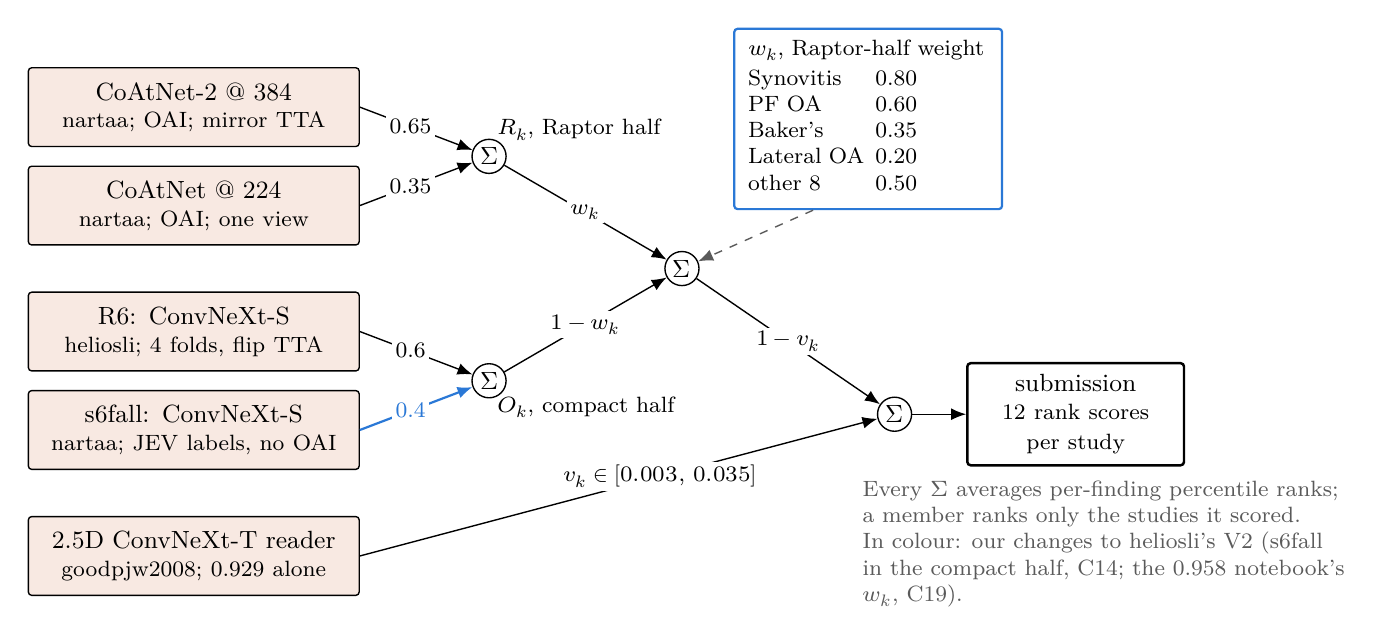
\begin{tikzpicture}[font=\small]
\tikzset{m/.style={pubm, text width=3.85cm, minimum height=1.0cm}, e/.style={font=\footnotesize, fill=paper, inner sep=1.2pt}}
% members
\node[m] (r384) at (0,3.3)  {CoAtNet-2 @ 384\\[-1pt]{\footnotesize nartaa; OAI; mirror TTA}};
\node[m] (r224) at (0,2.05) {CoAtNet @ 224\\[-1pt]{\footnotesize nartaa; OAI; one view}};
\node[m] (r6)   at (0,0.45) {R6: ConvNeXt-S\\[-1pt]{\footnotesize heliosli; 4 folds, flip TTA}};
\node[m] (s6)   at (0,-0.8) {s6fall: ConvNeXt-S\\[-1pt]{\footnotesize nartaa; JEV labels, no OAI}};
\node[m] (rd)   at (0,-2.4) {2.5D ConvNeXt-T reader\\[-1pt]{\footnotesize goodpjw2008; 0.929 alone}};
% raptor half and compact half
\node[op] (R) at (3.75,2.675) {$\Sigma$};
\node[op] (O) at (3.75,-0.175) {$\Sigma$};
\draw[flow] (r384.east) -- node[e, pos=0.45] {0.65} (R);
\draw[flow] (r224.east) -- node[e, pos=0.45] {0.35} (R);
\draw[flow] (r6.east) -- node[e, pos=0.45] {0.6} (O);
\draw[flow, own, line width=0.8pt] (s6.east) -- node[e, pos=0.45, text=own] {0.4} (O);
\node[anchor=south west, font=\footnotesize, inner sep=1pt] at ([xshift=-1mm]R.north east) {$R_k$, Raptor half};
\node[anchor=north west, font=\footnotesize, inner sep=1pt] at ([xshift=-1mm]O.south east) {$O_k$, compact half};
% per-finding mix
\node[op] (A) at (6.2,1.25) {$\Sigma$};
\draw[flow] (R) -- node[e, pos=0.5] {$w_k$} (A);
\draw[flow] (O) -- node[e, pos=0.5] {$1-w_k$} (A);
\node[blk, text width=3.05cm, align=left, anchor=west, font=\footnotesize, draw=own, line width=0.8pt] (wt) at (6.85,3.15) {%
$w_k$, Raptor-half weight\\[1pt]
\begin{tabular}{@{}l@{\hspace{4pt}}r@{}}
Synovitis & 0.80\\ PF OA & 0.60\\ Baker's & 0.35\\ Lateral OA & 0.20\\ other 8 & 0.50
\end{tabular}};
\draw[dflow] (wt.south) ++(-0.7,0) -- (A);
% final with the reader
\node[op] (F) at (8.9,-0.6) {$\Sigma$};
\draw[flow] (A) -- node[e, pos=0.5] {$1-v_k$} (F);
\draw[flow] (rd.east) -- node[e, pos=0.58] {$v_k\in[0.003,\,0.035]$} (F);
\node[blk, text width=2.4cm, line width=0.9pt] (sub) at (11.2,-0.6) {submission\\[-1pt]{\footnotesize 12 rank scores per study}};
\draw[flow] (F) -- (sub);
\node[note, anchor=north west, align=left] at (8.45,-1.4) {Every $\Sigma$ averages per-finding percentile ranks;\\a member ranks only the studies it scored.\\In colour: our changes to heliosli's V2 (s6fall\\in the compact half, C14; the 0.958 notebook's\\$w_k$, C19).};
\end{tikzpicture}
\end{document}
